\documentclass{article}

% Useful packages
\usepackage[letterpaper,top=2cm,bottom=2cm,left=3cm,right=3cm,marginparwidth=1.75cm]{geometry}
\usepackage{amsmath}
\usepackage{graphicx}
\usepackage[colorlinks=true, allcolors=blue]{hyperref}
\usepackage{titling}
\usepackage{float}
\usepackage[demo]{graphicx}
\usepackage[T1]{fontenc}
\usepackage[spanish]{babel}
\usepackage{tabularx}


% Useful for augmented matrix representation
\makeatletter
\renewcommand*\env@matrix[1][*\c@MaxMatrixCols c]{%
  \hskip -\arraycolsep
  \let\@ifnextchar\new@ifnextchar
  \array{#1}}
\makeatother

\usepackage{listings}
\usepackage{color}

\definecolor{dkgreen}{rgb}{0,0.6,0}
\definecolor{gray}{rgb}{0.5,0.5,0.5}
\definecolor{mauve}{rgb}{0.58,0,0.82}

\lstset{frame=tb,
  language=Matlab,
  aboveskip=3mm,
  belowskip=3mm,
  showstringspaces=false,
  columns=flexible,
  basicstyle={\small\ttfamily},
  numbers=none,
  numberstyle=\tiny\color{gray},
  keywordstyle=\color{blue},
  commentstyle=\color{dkgreen},
  stringstyle=\color{mauve},
  breaklines=true,
  breakatwhitespace=true,
  tabsize=3
}

\setcounter{section}{0}

\title{
\includegraphics[scale=0.5]{logo.jpg}\\ \textbf{Laboratorio 4} 
\\ \large RESOLUCIÓN DE UNA ECUACIÓN NO LINEAL           
\\ \large Métodos de Computación Científica}

\author{Manuel Lagos}

\begin{document}
\setcounter{section}{0}
\maketitle

\section{Ejercicio 1}
1.1 ¿Cómo se comporta el método de Newton con punto inicial $x_0 = 1$ cuando se lo aplica
para encontrar una solución de la siguiente ecuación no lineal:
\[x^5-x^3-4 \cdot x=0\]

Método de Newton-Raphson:
\vspace{0.5cm}\\
por taylor sabemos que
\[f(x+h) = f(x) + f^{'}(x) \cdot h\]
sea $x = x_k$, $h = x_{k+1} - x_k$ y $f(x_{k+1}) = 0$, es decir $x_{k+1}$ una raíz de $f$.
\[f(x_k + (x_{k+1}-x_k)) = f(x_k) + f^{'}(x_k) \cdot (x_{k+1}-x_k)\]
\[f(x_{k+1}) = f(x_k) + f^{'}(x_k) \cdot (x_{k+1}-x_k)\]
\[0 = f(x_k) + f^{'}(x_k) \cdot (x_{k+1}-x_k)\]
despejando $x_{k+1}$, si $f^{'}(x_k) \ne 0$ entonces
\[x_{k+1}=x_k + \dfrac{-f(x_k)}{f^{'}(x_k)}\]

sea $g(x) = x^5-x^3-4 \cdot x$,\\
\[
g^{'}(x) = 5\cdot x^4 -3 \cdot x^2 - 4
\]
si aplicamos el método partiendo de $x_0=1$ tenemos que:

\begin{table}[H]
\centering
\begin{tabular}{|l|l|l|l|l|}
\hline
$k$ & $x_k$ & $f(x_k)$ & $f^{'}(x_k)$ & $x_{k+1}$ \\ \hline
0 & 1    & -4      & -2                             & -1     \\ \hline
1 & -1   & 4       & -2                             & 1      \\ \hline
2 & 1    & -4      & -2                             & -1     \\ \hline
\end{tabular}
\end{table}

Como se observa ya en las primeras dos iteraciones de la tabla, \textbf{el método de newton para esta función y $x_0$ dados oscila} indefinidamente sin llegar a la solución.\\

1.2 ¿Cuáles son las raíces reales de la ecuación anterior? ¿Hay algo anómalo relacionado con
ellas?

Las raíces reales del polinomio son $x=0$, $x=\sqrt{\dfrac{1}{2}+\dfrac{\sqrt{17}}{2}}$, $x=-\sqrt{\dfrac{1}{2}+\dfrac{\sqrt{17}}{2}}$, y las complejas $x=i \cdot \sqrt{\dfrac{1}{2} \cdot (\sqrt{17} - 1)}$ y $x=-i \cdot \sqrt{\dfrac{1}{2} \cdot (\sqrt{17} - 1)}$.

\begin{figure}[H]
    \centering
    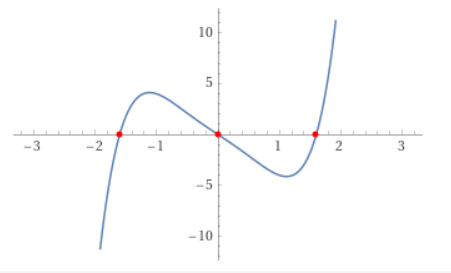
\includegraphics[width=0.7\linewidth]{Screenshot_20231111_154229.png}
    \label{fig:enter-label}
    \caption{Gráfica del polinomio $x^5-x^3-4 \cdot x$ en el plano real}
\end{figure}

\begin{figure}[H]
    \centering
    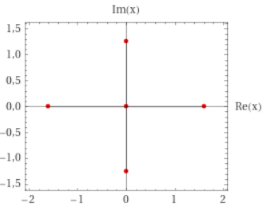
\includegraphics[width=0.3\linewidth]{Screenshot_20231111_154228.png}
    \label{fig:enter-label}
    \caption{Raíces del polinomio $x^5-x^3-4 \cdot x$ en el plano complejo}
\end{figure}

Notese que la función está espejada con respecto a una recta oblicua símil a $f(x)=-4x$, y la derivada en $x=1$ y $x=-1$ coinciden. La única diferencia entre un punto y el otro es el signo, esto hace que el método alterne entre un punto y otro cambiando el signo, luego diverge.  
\section{Ejercicio 2}
2.1 Emplee el método de Newton implementando un .m (script) para resolver lo siguiente:\\
a) $x^4 - x = 10$ (dos raíces reales y dos raíces complejas)\\
b) $e^{-x} = sin(x)$ (infinitamente muchas raíces)\\
c) $x^{3} - 8 \cdot x^2 + 17 \cdot x - 10 = 0$ (tres raíces reales)\\
d) $log(x) = cos(x)$\\
e) $x^{4} - 5 \cdot x^3 - 12 \cdot x^2 + 76 \cdot x - 79 = 0$ (cuatro raíces reales)\\
Ayuda: use fplot para tener una idea de dónde están las raíces.
2.2 Chequee sus respuestas con el comando fzero
2.3 Chequee sus respuestas que involucran ecuaciones polinomiales con el comando roots\\

Se desarrolló un programa en Octave para implementar el método de Newton-Raphson. A continuación los resultados obtenidos para cada función. 

\[a) x^4 - x -10 = 0\]
\begin{figure}[H]
    \centering
    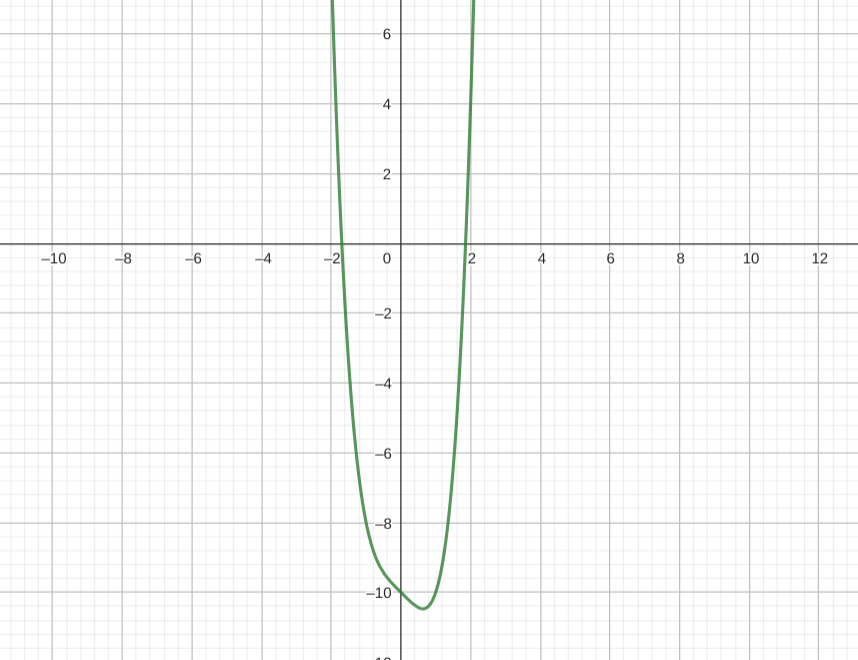
\includegraphics[width=0.65\linewidth]{a.png}
    \label{fig:enter-label}
    \caption{}
\end{figure}
\begin{lstlisting}
APROXIMACION CON EL METODO DE NEWTON-RAPHSON
funcion a buscar ceros: @(x) x .^ 4 - x - 10

a partir de x_0 inicial: -2
cantidad de iteraciones: 10
tiempo de ejecucion en segundos: 1.503944396972656e-03
resultado: -1.697471880844155
error absoluto: 0
resultado de fzero: -1.697471880844155
tiempo de ejecucion de fzero en segundos: 2.103090286254883e-03
diferencia con fzero: 0

a partir de x_0 inicial: 2
cantidad de iteraciones: 100000
tiempo de ejecucion en segundos: 4.222615003585815
resultado: 1.855584528640938
error absoluto: 1.776356839400250e-15
resultado de fzero: 1.855584528640938
tiempo de ejecucion de fzero en segundos: 2.032041549682617e-03
diferencia con fzero: 0   

a partir de x_0 inicial:  0 - 2i
cantidad de iteraciones: 10
tiempo de ejecucion en segundos: 1.479148864746094e-03
resultado: -7.905632389839126e-02 - 1.780042771099175e+00i

a partir de x_0 inicial:  0 + 2i
cantidad de iteraciones: 10
tiempo de ejecucion en segundos: 5.118846893310547e-04
resultado: -7.905632389839126e-02 + 1.780042771099175e+00i
error absoluto: 2.220446049250313e-16
\end{lstlisting}

\[b) e^{-x}-sin(x) = 0\]
\begin{figure}[H]
    \centering
    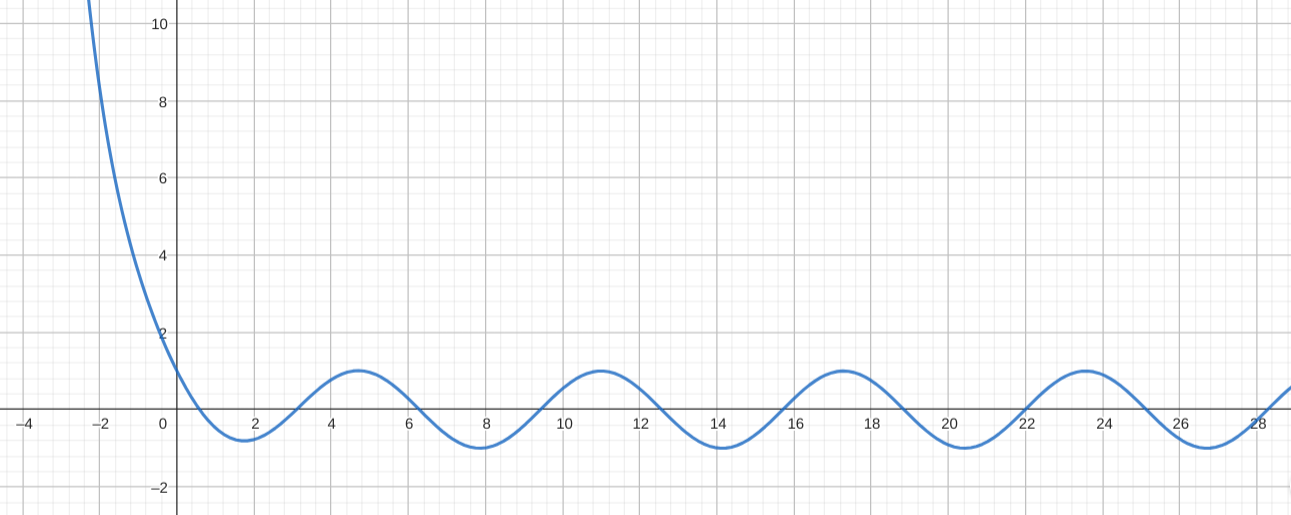
\includegraphics[width=0.9\linewidth]{b.png}
    \label{fig:enter-label}
    \caption{}
\end{figure}
\begin{lstlisting}
APROXIMACION CON EL METODO DE NEWTON-RAPHSON
funcion a buscar ceros: @(x) e ^ (-x) - sin (x)

a partir de x_0 inicial: 0
cantidad de iteraciones: 10
tiempo de ejecucion en segundos: 1.941919326782227e-03
resultado: 0.588532743981861
error absoluto: 0
resultado de fzero: 0.588532743981861
tiempo de ejecucion de fzero en segundos: 5.029916763305664e-03
diferencia con fzero: 0

a partir de x_0 inicial: 3
cantidad de iteraciones: 6
tiempo de ejecucion en segundos: 1.418113708496094e-03
resultado: 3.096363932410646
error absoluto: 1.110223024625157e-16
resultado de fzero: 3.096363932410644
tiempo de ejecucion de fzero en segundos: 4.950046539306641e-03
diferencia con fzero: 2.220446049250313e-15

a partir de x_0 inicial: 6
cantidad de iteraciones: 6
tiempo de ejecucion en segundos: 6.530284881591797e-04
resultado: 6.285049273382587
error absoluto: 1.422473250300982e-16
resultado de fzero: 6.285049273382582
tiempo de ejecucion de fzero en segundos: 2.447843551635742e-03
diferencia con fzero: 4.440892098500626e-15

a partir de x_0 inicial: 9
cantidad de iteraciones: 100000
tiempo de ejecucion en segundos: 6.857232093811035
resultado: 9.424697254738522
error absoluto: 7.151804105529069e-16
resultado de fzero: 9.424697254738517
tiempo de ejecucion de fzero en segundos: 1.969814300537109e-03
diferencia con fzero: 5.329070518200751e-15
\end{lstlisting}

\[c) x^3 -8x^2 +17x -10 = 0\]
\begin{figure}[H]
    \centering
    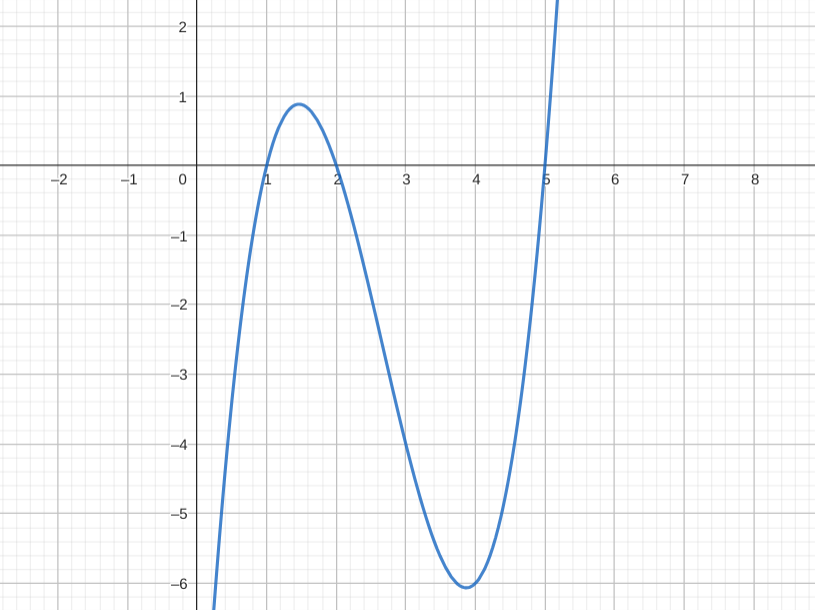
\includegraphics[width=0.8\linewidth]{c.png}
    \label{fig:enter-label}
    \caption{}
\end{figure}

\begin{lstlisting}
APROXIMACION CON EL METODO DE NEWTON-RAPHSON
funcion a buscar ceros: @(x) x .^ 3 - 8 * x .^ 2 + 17 * x - 10

a partir de x_0 inicial: 0.500000000000000
cantidad de iteraciones: 14
tiempo de ejecucion en segundos: 1.074075698852539e-03
resultado: 1
error absoluto: 0
resultado de fzero: 1
tiempo de ejecucion de fzero en segundos: 2.614021301269531e-03
diferencia con fzero: 0  

a partir de x_0 inicial: 1.600000000000000
cantidad de iteraciones: 12
tiempo de ejecucion en segundos: 3.386974334716797e-03
resultado: 2
error absoluto: 0
resultado de fzero: 2.000000000000000
tiempo de ejecucion de fzero en segundos: 8.651971817016602e-03
diferencia con fzero: 4.440892098500626e-16

a partir de x_0 inicial: 4.600000000000000
cantidad de iteraciones: 10
tiempo de ejecucion en segundos: 6.911754608154297e-04
resultado: 5.000000000000001
error absoluto: 0
resultado de fzero: 5.000000000000001
tiempo de ejecucion de fzero en segundos: 2.156019210815430e-03
diferencia con fzero: 0
\end{lstlisting}

\[d) log(x) - cos(x) = 0\]
\begin{figure}[H]
    \centering
    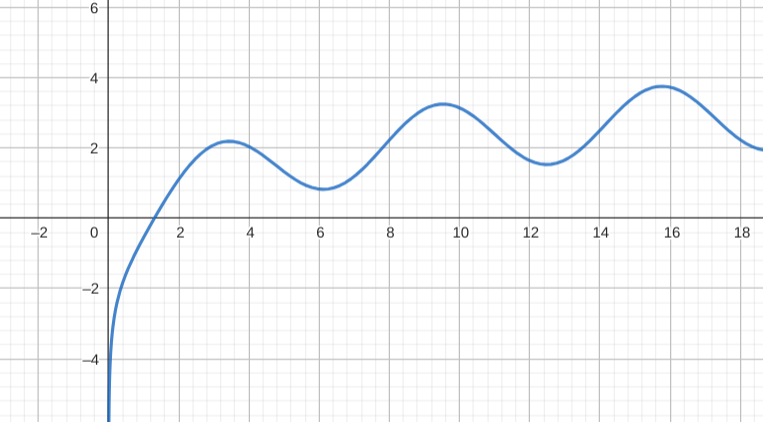
\includegraphics[width=0.7\linewidth]{d.png}
    \label{fig:enter-label}
    \caption{}
\end{figure}

\begin{lstlisting}
APROXIMACION CON EL METODO DE NEWTON-RAPHSON
funcion a buscar ceros: @(x) log (x) - cos (x)
a partir de x_0 inicial: 1
cantidad de iteraciones: 8
tiempo de ejecucion en segundos: 6.930828094482422e-04
resultado: 1.302964001216013
error absoluto: 1.665334536937735e-16
resultado de fzero: 1.302964001216012
tiempo de ejecucion de fzero en segundos: 3.302812576293945e-03
diferencia con fzero: 1.110223024625157e-15
\end{lstlisting}

\vspace{10cm}

\[e) x^4 - 5 \cdot x^3 - 12 \cdot x^2 +76 \cdot x -79 = 0\]
\begin{figure}[H]
    \centering
    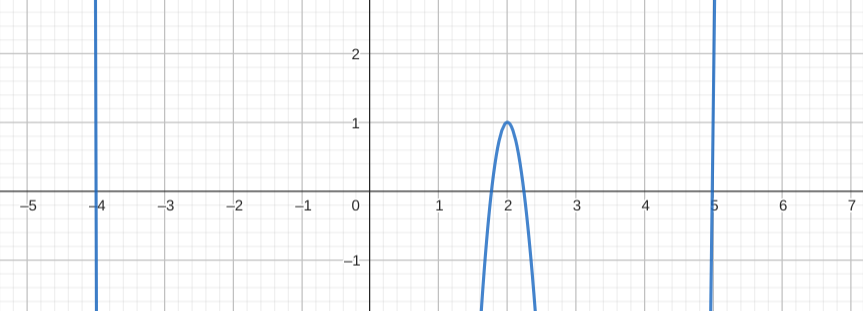
\includegraphics[width=0.7\linewidth]{e.png}
    \label{fig:enter-label}
    \caption{}
\end{figure}

\begin{lstlisting}
APROXIMACION CON EL METODO DE NEWTON-RAPHSON
funcion a buscar ceros: @(x) x .^ 4 - 5 * x .^ 3 - 12 * x .^ 2 + 76 * x - 79

a partir de x_0 inicial: -4
cantidad de iteraciones: 8
tiempo de ejecucion en segundos: 5.080699920654297e-04
resultado: -3.996909336738181
error absoluto: 0
resultado de fzero: -3.996909336738184
tiempo de ejecucion de fzero en segundos: 1.466989517211914e-03
diferencia con fzero: 2.220446049250313e-15

a partir de x_0 inicial: 1.500000000000000
cantidad de iteraciones: 16
tiempo de ejecucion en segundos: 9.720325469970703e-04
resultado: 1.768386894910355
error absoluto: 0
resultado de fzero: 1.768386894910352
tiempo de ejecucion de fzero en segundos: 2.944946289062500e-03
diferencia con fzero: 3.552713678800501e-15

a partir de x_0 inicial: 2.500000000000000
cantidad de iteraciones: 100000
tiempo de ejecucion en segundos: 4.778645992279053
resultado: 2.240988633661078
error absoluto: 1.421085471520200e-14
resultado de fzero: 2.240988633661078
tiempo de ejecucion de fzero en segundos: 2.466917037963867e-03
diferencia con fzero: 4.440892098500626e-16

a partir de x_0 inicial: 5
cantidad de iteraciones: 6
tiempo de ejecucion en segundos: 1.014947891235352e-03
resultado: 4.987533808166751
error absoluto: 0
resultado de fzero: 4.987533808166753
tiempo de ejecucion de fzero en segundos: 4.945039749145508e-03
diferencia con fzero: 1.776356839400250e-15
\end{lstlisting}

\vspace{2cm}

\[
\textbf{Código del programa para Newton-Raphson}
\]
\begin{lstlisting}
    % limpiar la consola
clc;

function dfdx = difcentr(f, x)
    h = sqrt(eps); % segun la regla del pulgar
    dfdx = (f(x+h)-f(x-h))/(2*h);
end

function [siguiente, i] = newton(f, anterior, ITERACIONES, TOL)
    i = 0;
    siguiente = anterior;

    while (abs(f(anterior)) > TOL && i < ITERACIONES)
      aux = siguiente;
      siguiente = anterior - f(anterior)/difcentr(f, anterior);
      anterior = aux;
      i += 1;
    end
end

% constantes para criterio de parada
ITERACIONES = 100000;
TOL = eps;

% funciones
% f = @(x) x.^4 - x - 10;
% f = @(x) e^(-x) - sin(x);
% f = @(x) x.^3 - 8*x.^2 + 17*x - 10;
% f = @(x) log(x)-cos(x);
% f = @(x) x.^4 - 5*x.^3 - 12*x.^2 + 76 * x - 79;

% f = @(x) x.^3 -2*x - 5;
% f = @(x) e.^(-x) - x;
% f = @(x) x * sin(x) - 1;
% f = @(x) x.^3 -3*x.^2+3*x-1;

% funcion a obtener f(x) = 0
f = @(x) x.^3 -3*x.^2+3*x-1;

% aproximacion incial
inicial = 0;

% calcular aproximacion
tic; % empezar a medir el tiempo
[res, i]= newton(f, inicial, ITERACIONES, TOL);
time = toc; % obtener el tiempo de ejecucion

format long;
printf("APROXIMACION CON EL METODO DE NEWTON-RAPHSON \n");

% mostrar funcion
printf("funcion a buscar ceros: ");
disp(f);

% mostrar x_0 inicial
printf("a partir de x_0 inicial: ");
disp(inicial);

% mostrar cantidad de iteraciones
printf("cantidad de iteraciones: ");
disp(i);

% mostrar tiempo de ejecucion
printf("tiempo de ejecucion en segundos: ");
disp(time)

% mostrar error
printf("resultado: ");
disp(res(1));

% mostrar resultado
printf("error absoluto: ");
disp(abs(f(res)));

% mostrar resultado con fzero
printf("resultado de fzero: ");

tic;
fz = fzero(f, inicial);
time = toc;

disp(fz);

% mostrar tiempo de ejecucion de fzero
printf("tiempo de ejecucion de fzero en segundos: ");
disp(time)

% diferencia resultado con fzero
printf("diferencia con fzero: ");
disp(abs(res - fz));
\end{lstlisting}

\section{Ejercicio 3}
Implemente los métodos de Bisección, Newton y Secante para resolver
ecuaciones no lineales en una dimensión y testee sus implementaciones encontrando por lo
menos una raíz de cada una de las siguientes ecuaciones:\\
a) $x^{3} - 2 \cdot x - 5 = 0$ \\
b) $e^{-x} - x = 0$ \\
c) $x \cdot sin(x) -1 = 0$ \\
d) $x^{3} - 3 \cdot x^{2} + 3 \cdot x - 1 = 0$ \\
3.1 Qué criterio de terminación debería usar?\\
3.2 Qué velocidad de convergencia se logra en cada caso?\\
3.3 Compare sus resultados (las soluciones y velocidades de convergencia) con aquellos
provenientes de alguna rutina ofrecida por las librerías de Matlab u Octave para resolver
ecuaciones no lineales.\\

Se impletaron los métodos de Bisección, Newton y Secante en Octave. A continuación se presentan los gráficos y los resultados obtenidos para cada función y para cada punto inicial. Además se comparó el tiempo de ejecución obtenido por el algoritmo con el de la rutina fzero/roots ofrecidas en la liberría de Octave. Al final del ejercicio se ecuentra el código. \\

\vspace{4cm}

a)
\[ x^{3} - 2 \cdot x - 5 = 0\]

\begin{lstlisting}
APROXIMACION CON EL METODO DE BISECCION
funcion a buscar ceros: @(x) x .^ 3 - 2 * x - 5
intervalo a buscar ceros: [1, 3]
cantidad de iteraciones: 100000
tiempo de ejecucion en segundos: 2.183656930923462
resultado: 2.094551481542327
error absoluto: 3.552713678800501e-15
resultado de fzero: 2.094551481542328
diferencia con fzero: 1.332267629550188e-15

APROXIMACION CON EL METODO DE NEWTON-RAPHSON
funcion a buscar ceros: @(x) x .^ 3 - 2 * x - 5
a partir de x_0 inicial: 2
cantidad de iteraciones: 100000
tiempo de ejecucion en segundos: 4.471329927444458
resultado: 2.094551481542327
error absoluto: 8.881784197001252e-16
resultado de fzero: 2.094551481542328
tiempo de ejecucion de fzero en segundos: 1.953125000000000e-03
diferencia con fzero: 1.776356839400250e-15

APROXIMACION CON EL METODO DE LA SECANTE
funcion a buscar ceros: @(x) x .^ 3 - 2 * x - 5
intervalo a buscar ceros: [1, 3]
cantidad de iteraciones: 100000
tiempo de ejecucion en segundos: 2.771811962127686
resultado: 3.618033988749885
error absoluto: 35.12461179749773
resultado de fzero: 2.094551481542328
diferencia con fzero: 1.523482507207556
(el método oscila)
\end{lstlisting}

b)
\[ e^{-x} - x = 0\]
\begin{lstlisting}
APROXIMACION CON EL METODO DE BISECCION
funcion a buscar ceros: @(x) e .^ (-x) - x
intervalo a buscar ceros: [0, 1]
cantidad de iteraciones: 50
tiempo de ejecucion en segundos: 4.005908966064453e-03
resultado: 0.567143290409784
error absoluto: 1.110223024625157e-16
resultado de fzero: 0.567143290409785
diferencia con fzero: 5.551115123125783e-16

APROXIMACION CON EL METODO DE NEWTON-RAPHSON
funcion a buscar ceros: @(x) e .^ (-x) - x
a partir de x_0 inicial: 0
cantidad de iteraciones: 10
tiempo de ejecucion en segundos: 1.800060272216797e-03
resultado: 0.567143290409784
error absoluto: 1.110223024625157e-16
resultado de fzero: 0.567143290409783
tiempo de ejecucion de fzero en segundos: 5.698919296264648e-03
diferencia con fzero: 5.551115123125783e-16

APROXIMACION CON EL METODO DE LA SECANTE
funcion a buscar ceros: @(x) e .^ (-x) - x
intervalo a buscar ceros: [0, 1]
cantidad de iteraciones: 100000
tiempo de ejecucion en segundos: 3.805847883224487
resultado: 0.567143290409784
error absoluto: 1.110223024625157e-16
resultado de fzero: 0.567143290409785
diferencia con fzero: 5.551115123125783e-16
\end{lstlisting}

c)
\[ x \cdot sin(x) - 1 = 0\]
\begin{lstlisting}
APROXIMACION CON EL METODO DE BISECCION
funcion a buscar ceros: @(x) x * sin (x) - 1
intervalo a buscar ceros: [0, 2]
cantidad de iteraciones: 52
tiempo de ejecucion en segundos: 5.002021789550781e-03
resultado: 1.114157140871930
error absoluto: 2.220446049250313e-16
resultado de fzero: 1.114157140871929
diferencia con fzero: 1.110223024625157e-15   

APROXIMACION CON EL METODO DE NEWTON-RAPHSON
funcion a buscar ceros: @(x) x * sin (x) - 1
a partir de x_0 inicial: 1
cantidad de iteraciones: 6
tiempo de ejecucion en segundos: 5.168914794921875e-04
resultado: 1.114157140871930
error absoluto: 2.220446049250313e-16
resultado de fzero: 1.114157140871929
tiempo de ejecucion de fzero en segundos: 2.329111099243164e-03
diferencia con fzero: 8.881784197001252e-16

APROXIMACION CON EL METODO DE LA SECANTE
funcion a buscar ceros: @(x) x * sin (x) - 1
intervalo a buscar ceros: [0, 2]
cantidad de iteraciones: 100000
tiempo de ejecucion en segundos: 3.838794946670532
resultado: 1.114157140871930
error absoluto: 2.220446049250313e-16
resultado de fzero: 1.114157140871929
diferencia con fzero: 8.881784197001252e-16
\end{lstlisting}

d)
\[ x^{3} -3 \cdot x^{2} + 3 \cdot x - 1 = 0\]
\begin{lstlisting}
APROXIMACION CON EL METODO DE BISECCION
funcion a buscar ceros: @(x) x .^ 3 - 3 * x .^ 2 + 3 * x - 1
intervalo a buscar ceros: [0, 2]
cantidad de iteraciones: 0
tiempo de ejecucion en segundos: 1.039505004882812e-04
resultado: 1
error absoluto: 0
resultado de fzero: 1
diferencia con fzero: 0

APROXIMACION CON EL METODO DE NEWTON-RAPHSON
funcion a buscar ceros: @(x) x .^ 3 - 3 * x .^ 2 + 3 * x - 1
a partir de x_0 inicial: 0
cantidad de iteraciones: 52
tiempo de ejecucion en segundos: 6.027936935424805e-03
resultado: Inf
error absoluto: NaN
resultado de fzero: 1.000003854250249
tiempo de ejecucion de fzero en segundos: 1.132798194885254e-02
diferencia con fzero: Inf
(el método diverge)

APROXIMACION CON EL METODO DE LA SECANTE
funcion a buscar ceros: @(x) x .^ 3 - 3 * x .^ 2 + 3 * x - 1
intervalo a buscar ceros: [0, 2]
cantidad de iteraciones: 100000
tiempo de ejecucion en segundos: 2.946841955184937
resultado: 1
error absoluto: 0
resultado de fzero: 1
diferencia con fzero: 0
\end{lstlisting}

\[
\textbf{Código del programa para el método de Bisección}
\]
\begin{lstlisting}
% limpiar la consola
clc;

function [res, i] = bisecc(f, a, b, ITERACIONES, TOL)
    i = 0;
    res = a + ((b-a)./2);

    while (abs(f(res)) > TOL && i < ITERACIONES)
      res = a + ((b-a)./2);

      if (f(a) * f(res) > 0)
        a = res;
      else
        b = res;
      end

      i += 1;
    end
end

% constantes para criterio de parada
ITERACIONES = 100000;
TOL = eps;

% funciones
% f = @(x) x.^3 -2*x - 5;
% f = @(x) e.^(-x) - x;
% f = @(x) x * sin(x) - 1;
% f = @(x) x.^3 -3*x.^2+3*x-1;

% funcion a obtener f(x) = 0
f = @(x) x.^3 -3*x.^2+3*x-1;

% aproximacion incial
a = 0;
b = 2;

% calcular aproximacion
tic; % empezar a medir el tiempo
[res, i]= bisecc(f, a, b, ITERACIONES, TOL);
time = toc; % obtener el tiempo de ejecucion

format long;
printf("APROXIMACION CON EL METODO DE BISECCION \n");

% mostrar funcion
printf("funcion a buscar ceros: ");
disp(f);

% mostrar invervalo
printf("intervalo a buscar ceros: [%d, %d]\n", a, b);

% mostrar cantidad de iteraciones
printf("cantidad de iteraciones: ");
disp(i);

% mostrar tiempo de ejecucion
printf("tiempo de ejecucion en segundos: ");
disp(time)

% mostrar error
printf("resultado: ");
disp(res(1));

% mostrar resultado
printf("error absoluto: ");
disp(abs(f(res)));

% mostrar resultado con fzero
printf("resultado de fzero: ");
disp(fzero(f, (b-a)/2));

% diferencia resultado con fzero
printf("diferencia con fzero: ");
disp(abs(res - fzero(f, (b-a)/2)));    
\end{lstlisting}

\[
\textbf{Código del programa para Secante}
\]
\begin{lstlisting}
% limpiar la consola
clc;

function [siguiente, i] = secant(f, anterior, siguiente, ITERACIONES, TOL)
    i = 0;

    while (abs(f(anterior)) > TOL && i < ITERACIONES)
      p = (f(siguiente)-f(anterior))/(siguiente-anterior);
      siguiente = anterior - (f(anterior)./p);
      i += 1;
    end
end

% constantes para criterio de parada
ITERACIONES = 100000;
TOL = eps;

% funciones
% f = @(x) x.^3 -2*x - 5;
% f = @(x) e.^(-x) - x;
% f = @(x) x * sin(x) - 1;
% f = @(x) x.^3 -3*x.^2+3*x-1;

% funcion a obtener f(x) = 0
f = @(x) x.^3 -3*x.^2+3*x-1;

% aproximacion incial
anterior = 0;
siguiente = 2;

% calcular aproximacion
tic; % empezar a medir el tiempo
[res, i]= secant(f, anterior, siguiente, ITERACIONES, TOL);
time = toc; % obtener el tiempo de ejecucion

format long;
printf("APROXIMACION CON EL METODO DE LA SECANTE \n");

% mostrar funcion
printf("funcion a buscar ceros: ");
disp(f);

% mostrar invervalo
printf("intervalo a buscar ceros: [%d, %d]\n", anterior, siguiente);

% mostrar cantidad de iteraciones
printf("cantidad de iteraciones: ");
disp(i);

% mostrar tiempo de ejecucion
printf("tiempo de ejecucion en segundos: ");
disp(time)

% mostrar error
printf("resultado: ");
disp(res(1));

% mostrar resultado
printf("error absoluto: ");
disp(abs(f(res)));

% mostrar resultado con fzero
printf("resultado de fzero: ");
disp(fzero(f, siguiente));

% diferencia resultado con fzero
printf("diferencia con fzero: ");
disp(abs(res - fzero(f, siguiente)));    
\end{lstlisting}
\textit{
Para el método de Newton se usó el mísmo programa del ejercicio 2.}

Según fue visto en la teoría, el método de Newton tiene un orden de convergencia cuadrático con una constante $C = \dfrac{1}{2}$, el método de Bisección un orden lineal con $C = \dfrac{1}{2} \cdot \dfrac{|f^{''}(\alpha)|}{|f^{'}(\alpha)|}$, y el método de la secante un orden superineal ($p = 1.62$) y $C = {(\dfrac{1}{2} \cdot \dfrac{|f^{''}(\alpha)|}{|f^{'}(\alpha)|})}^{0.62}$. Por lo que es esperable que el tiempo de ejecución del método de Newton sea menor.

\section{Ejercicio 4}
Para la ecuación: $f(x) = x^2 - 3\cdot x + 2 = 0$, cada una de las siguientes
funciones brinda un problema equivalente de punto fijo:
\[g_1(x)=\dfrac{(x^2+2)}{3}\]
\[g_2(x)=\sqrt{3\cdot x -2}\]
4.1 Analice las propiedades de convergencia correspondientes a cada uno de los esquemas
de punto fijo de iteración, es decir $x{k+1} = g_i(x_k)$ con $i = 1,2$ para la raíz $x = 2$, mediante
el estudio de $|g_i^{'}(2)|$\\

El método de punto fijo converge para una $g(x)=x$ dado un $x_0$ inicial si y solo si $|g^{'}(x_0)|<1$, y converge relativamente más rápido cuanto más cercano a sea dicha expresión a 0.\\
\[g_1^{'}(x) = \dfrac{2 \cdot x}{3}\]
\[|g_1^{'}(2)| = |\dfrac{4}{3}| = \dfrac{4}{3} > 1\]
luego, el método con $g_1(x)$ a partir de $x=2$ diverge.
\[g_2^{'}(x) = \dfrac{3}{2\cdot \sqrt{3 \cdot x - 2}}\]
\[|g_2^{'}(2)| = |\dfrac{3}{2\cdot \sqrt{3 \cdot 2 - 2}}| = |\dfrac{3}{2\cdot \sqrt{4}}| = |\dfrac{3}{4}| = \dfrac{3}{4} < 1\]
luego, el método con $g_2(x)$ a partir de $x=2$ converge.\\

4.2 Confirme su análisis implementando cada uno de los esquemas y verificando su
convergencia (o su divergencia) y el orden aproximado de convergencia.\\

Se implementó en Octave el método de punto fijo a partir de una $g(x)=x$ y un $x_0$ inicial. Este mismo se probó para las funciones $g_1$ y $g_2$ dadas, y se eligió $x_0=2+10^{-10}$ como aproximación inicial, dado que no tiene sentido elegir $x_0=2$ ya que esta es una de las soluciones en primer lugar, lo cual en el mundo real no suele ser el caso, desafortunadamente. A continuación los resultados obtenidos y el código del programa.\\

\begin{lstlisting}
APROXIMACION CON EL METODO DE PUNTO FIJO
funcion a buscar f(x)=x: @(x) (x .^ 2 + 2) / 3
cantidad de iteraciones: 91
tiempo de ejecucion en segundos: 4.348993301391602e-03
resultado: Inf
error absoluto: NaN
\end{lstlisting}
Efectivamente, el método diverge para $g_1$ con $x_0$ cercano a $2$.
\begin{lstlisting}
APROXIMACION CON EL METODO DE PUNTO FIJO
funcion a buscar f(x)=x: @(x) sqrt (3 * x - 2)
cantidad de iteraciones: 41
tiempo de ejecucion en segundos: 1.247882843017578e-03
resultado: 2.000000000000000
error absoluto: 0
\end{lstlisting}
Como se supuso, el método converge para $g_2$ con $x_0$ cercano a $2$.\\
\vspace{5cm}
\[
\textbf{Código del programa:}
\]
\begin{lstlisting}
% limpiar la consola
clc;

function [x, i] = pfijo(f, x, ITERACIONES, TOL)
    i = 0;
    while (abs(f(x)-x) > TOL && i < ITERACIONES)
      x = f(x);
      i += 1;
    end
end

% constantes para criterio de parada
ITERACIONES = 1000;
TOL = eps;

% funciones
% f = @(x) (x.^2+2)/3;
% f = @(x) sqrt(3*x-2);

% funcion a obtener f(x) = x
f = @(x) (x.^2+2)/3;

% aproximacion incial
inicial = 2 + 10.^-10;

% calcular aproximacion
tic; % empezar a medir el tiempo
[res, i]= pfijo(f, inicial, ITERACIONES, TOL);
time = toc; % obtener el tiempo de ejecucion

format long;
printf("APROXIMACION CON EL METODO DE PUNTO FIJO \n\n");

% mostrar funcion
printf("funcion a buscar f(x)=x: ");
disp(f);

% mostrar cantidad de iteraciones
printf("cantidad de iteraciones: ");
disp(i);

% mostrar tiempo de ejecucion
printf("tiempo de ejecucion en segundos: ");
disp(time)

% mostrar error
printf("resultado: ");
disp(res(1));

% mostrar resultado
printf("error absoluto: ");
disp(abs(f(res(1))-res(1)));
\end{lstlisting}
\end{document}